% Graphic for TeX using PGF
% Title: C:\Users\Ahmet\Desktop\testen\design1\design1.txt
% Creator: Dia v0.97.2
% CreationDate: Sun Jan 12 10:47:34 2020
% For: Ahmet
% \usepackage{tikz}
% The following commands are not supported in PSTricks at present
% We define them conditionally, so when they are implemented,
% this pgf file will use them.
\ifx\du\undefined
\newlength{\du}
\fi
\setlength{\du}{15\unitlength}
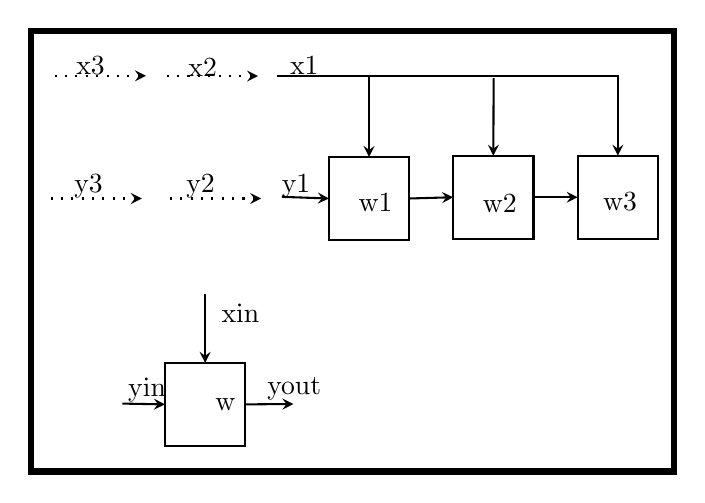
\begin{tikzpicture}
\pgftransformxscale{1.000000}
\pgftransformyscale{-1.000000}
\definecolor{dialinecolor}{rgb}{0.000000, 0.000000, 0.000000}
\pgfsetstrokecolor{dialinecolor}
\definecolor{dialinecolor}{rgb}{1.000000, 1.000000, 1.000000}
\pgfsetfillcolor{dialinecolor}
\pgfsetlinewidth{0.050000\du}
\pgfsetdash{}{0pt}
\pgfsetdash{}{0pt}
\pgfsetbuttcap
\pgfsetmiterjoin
\pgfsetlinewidth{0.050000\du}
\pgfsetbuttcap
\pgfsetmiterjoin
\pgfsetdash{}{0pt}
\definecolor{dialinecolor}{rgb}{1.000000, 1.000000, 1.000000}
\pgfsetfillcolor{dialinecolor}
\fill (15.732258\du,4.950000\du)--(15.732258\du,6.950000\du)--(17.667742\du,6.950000\du)--(17.667742\du,4.950000\du)--cycle;
\definecolor{dialinecolor}{rgb}{0.000000, 0.000000, 0.000000}
\pgfsetstrokecolor{dialinecolor}
\draw (15.732258\du,4.950000\du)--(15.732258\du,6.950000\du)--(17.667742\du,6.950000\du)--(17.667742\du,4.950000\du)--cycle;
\pgfsetbuttcap
\pgfsetmiterjoin
\pgfsetdash{}{0pt}
\definecolor{dialinecolor}{rgb}{0.000000, 0.000000, 0.000000}
\pgfsetstrokecolor{dialinecolor}
\draw (15.732258\du,4.950000\du)--(15.732258\du,6.950000\du)--(17.667742\du,6.950000\du)--(17.667742\du,4.950000\du)--cycle;
% setfont left to latex
\definecolor{dialinecolor}{rgb}{0.000000, 0.000000, 0.000000}
\pgfsetstrokecolor{dialinecolor}
\node[anchor=west] at (16.200000\du,6.050000\du){w1};
\pgfsetlinewidth{0.050000\du}
\pgfsetdash{}{0pt}
\pgfsetdash{}{0pt}
\pgfsetbuttcap
\pgfsetmiterjoin
\pgfsetlinewidth{0.050000\du}
\pgfsetbuttcap
\pgfsetmiterjoin
\pgfsetdash{}{0pt}
\definecolor{dialinecolor}{rgb}{1.000000, 1.000000, 1.000000}
\pgfsetfillcolor{dialinecolor}
\fill (18.725000\du,4.920000\du)--(18.725000\du,6.920000\du)--(20.660484\du,6.920000\du)--(20.660484\du,4.920000\du)--cycle;
\definecolor{dialinecolor}{rgb}{0.000000, 0.000000, 0.000000}
\pgfsetstrokecolor{dialinecolor}
\draw (18.725000\du,4.920000\du)--(18.725000\du,6.920000\du)--(20.660484\du,6.920000\du)--(20.660484\du,4.920000\du)--cycle;
\pgfsetbuttcap
\pgfsetmiterjoin
\pgfsetdash{}{0pt}
\definecolor{dialinecolor}{rgb}{0.000000, 0.000000, 0.000000}
\pgfsetstrokecolor{dialinecolor}
\draw (18.725000\du,4.920000\du)--(18.725000\du,6.920000\du)--(20.660484\du,6.920000\du)--(20.660484\du,4.920000\du)--cycle;
% setfont left to latex
\definecolor{dialinecolor}{rgb}{0.000000, 0.000000, 0.000000}
\pgfsetstrokecolor{dialinecolor}
\node[anchor=west] at (19.192742\du,6.070000\du){w2};
\pgfsetlinewidth{0.050000\du}
\pgfsetdash{}{0pt}
\pgfsetdash{}{0pt}
\pgfsetbuttcap
\pgfsetmiterjoin
\pgfsetlinewidth{0.050000\du}
\pgfsetbuttcap
\pgfsetmiterjoin
\pgfsetdash{}{0pt}
\definecolor{dialinecolor}{rgb}{1.000000, 1.000000, 1.000000}
\pgfsetfillcolor{dialinecolor}
\fill (21.725000\du,4.920000\du)--(21.725000\du,6.920000\du)--(23.660484\du,6.920000\du)--(23.660484\du,4.920000\du)--cycle;
\definecolor{dialinecolor}{rgb}{0.000000, 0.000000, 0.000000}
\pgfsetstrokecolor{dialinecolor}
\draw (21.725000\du,4.920000\du)--(21.725000\du,6.920000\du)--(23.660484\du,6.920000\du)--(23.660484\du,4.920000\du)--cycle;
\pgfsetbuttcap
\pgfsetmiterjoin
\pgfsetdash{}{0pt}
\definecolor{dialinecolor}{rgb}{0.000000, 0.000000, 0.000000}
\pgfsetstrokecolor{dialinecolor}
\draw (21.725000\du,4.920000\du)--(21.725000\du,6.920000\du)--(23.660484\du,6.920000\du)--(23.660484\du,4.920000\du)--cycle;
% setfont left to latex
\definecolor{dialinecolor}{rgb}{0.000000, 0.000000, 0.000000}
\pgfsetstrokecolor{dialinecolor}
\node[anchor=west] at (22.092742\du,6.020000\du){w3};
\pgfsetlinewidth{0.050000\du}
\pgfsetdash{}{0pt}
\pgfsetdash{}{0pt}
\pgfsetmiterjoin
\pgfsetbuttcap
{
	\definecolor{dialinecolor}{rgb}{0.000000, 0.000000, 0.000000}
	\pgfsetfillcolor{dialinecolor}
	% was here!!!
	\pgfsetarrowsend{stealth}
	{\pgfsetcornersarced{\pgfpoint{0.000000\du}{0.000000\du}}\definecolor{dialinecolor}{rgb}{0.000000, 0.000000, 0.000000}
		\pgfsetstrokecolor{dialinecolor}
		\draw (14.500000\du,3.010000\du)--(14.500000\du,3.000000\du)--(16.250000\du,3.000000\du)--(16.250000\du,3.000000\du)--(22.692742\du,3.000000\du)--(22.692742\du,4.920000\du);
}}
\pgfsetlinewidth{0.050000\du}
\pgfsetdash{}{0pt}
\pgfsetdash{}{0pt}
\pgfsetbuttcap
{
	\definecolor{dialinecolor}{rgb}{0.000000, 0.000000, 0.000000}
	\pgfsetfillcolor{dialinecolor}
	% was here!!!
	\pgfsetarrowsend{stealth}
	\definecolor{dialinecolor}{rgb}{0.000000, 0.000000, 0.000000}
	\pgfsetstrokecolor{dialinecolor}
	\draw (19.700000\du,3.050000\du)--(19.692742\du,4.920000\du);
}
\pgfsetlinewidth{0.050000\du}
\pgfsetdash{}{0pt}
\pgfsetdash{}{0pt}
\pgfsetbuttcap
{
	\definecolor{dialinecolor}{rgb}{0.000000, 0.000000, 0.000000}
	\pgfsetfillcolor{dialinecolor}
	% was here!!!
	\pgfsetarrowsend{stealth}
	\definecolor{dialinecolor}{rgb}{0.000000, 0.000000, 0.000000}
	\pgfsetstrokecolor{dialinecolor}
	\draw (16.700000\du,3.000000\du)--(16.700000\du,4.950000\du);
}
\pgfsetlinewidth{0.050000\du}
\pgfsetdash{}{0pt}
\pgfsetdash{}{0pt}
\pgfsetbuttcap
{
	\definecolor{dialinecolor}{rgb}{0.000000, 0.000000, 0.000000}
	\pgfsetfillcolor{dialinecolor}
	% was here!!!
	\pgfsetarrowsend{stealth}
	\definecolor{dialinecolor}{rgb}{0.000000, 0.000000, 0.000000}
	\pgfsetstrokecolor{dialinecolor}
	\draw (17.667742\du,5.950000\du)--(18.725000\du,5.920000\du);
}
\pgfsetlinewidth{0.050000\du}
\pgfsetdash{}{0pt}
\pgfsetdash{}{0pt}
\pgfsetbuttcap
{
	\definecolor{dialinecolor}{rgb}{0.000000, 0.000000, 0.000000}
	\pgfsetfillcolor{dialinecolor}
	% was here!!!
	\pgfsetarrowsend{stealth}
	\definecolor{dialinecolor}{rgb}{0.000000, 0.000000, 0.000000}
	\pgfsetstrokecolor{dialinecolor}
	\draw (20.660484\du,5.920000\du)--(21.725000\du,5.920000\du);
}
% setfont left to latex
\definecolor{dialinecolor}{rgb}{0.000000, 0.000000, 0.000000}
\pgfsetstrokecolor{dialinecolor}
\node[anchor=west] at (14.550000\du,2.760000\du){x1};
\pgfsetlinewidth{0.050000\du}
\pgfsetdash{}{0pt}
\pgfsetdash{}{0pt}
\pgfsetbuttcap
{
	\definecolor{dialinecolor}{rgb}{0.000000, 0.000000, 0.000000}
	\pgfsetfillcolor{dialinecolor}
	% was here!!!
	\pgfsetarrowsend{stealth}
	\definecolor{dialinecolor}{rgb}{0.000000, 0.000000, 0.000000}
	\pgfsetstrokecolor{dialinecolor}
	\draw (14.600000\du,5.910000\du)--(15.732258\du,5.950000\du);
}
% setfont left to latex
\definecolor{dialinecolor}{rgb}{0.000000, 0.000000, 0.000000}
\pgfsetstrokecolor{dialinecolor}
\node[anchor=west] at (14.350000\du,5.660000\du){y1};
\pgfsetlinewidth{0.050000\du}
\pgfsetdash{{\pgflinewidth}{0.200000\du}}{0cm}
\pgfsetdash{{\pgflinewidth}{0.200000\du}}{0cm}
\pgfsetbuttcap
{
	\definecolor{dialinecolor}{rgb}{0.000000, 0.000000, 0.000000}
	\pgfsetfillcolor{dialinecolor}
	% was here!!!
	\pgfsetarrowsend{stealth}
	\definecolor{dialinecolor}{rgb}{0.000000, 0.000000, 0.000000}
	\pgfsetstrokecolor{dialinecolor}
	\draw (11.900000\du,5.950000\du)--(14.100000\du,5.950000\du);
}
\pgfsetlinewidth{0.050000\du}
\pgfsetdash{{\pgflinewidth}{0.200000\du}}{0cm}
\pgfsetdash{{\pgflinewidth}{0.200000\du}}{0cm}
\pgfsetbuttcap
{
	\definecolor{dialinecolor}{rgb}{0.000000, 0.000000, 0.000000}
	\pgfsetfillcolor{dialinecolor}
	% was here!!!
	\pgfsetarrowsend{stealth}
	\definecolor{dialinecolor}{rgb}{0.000000, 0.000000, 0.000000}
	\pgfsetstrokecolor{dialinecolor}
	\draw (9.025000\du,5.950902\du)--(11.225000\du,5.950902\du);
}
\pgfsetlinewidth{0.050000\du}
\pgfsetdash{{\pgflinewidth}{0.200000\du}}{0cm}
\pgfsetdash{{\pgflinewidth}{0.200000\du}}{0cm}
\pgfsetbuttcap
{
	\definecolor{dialinecolor}{rgb}{0.000000, 0.000000, 0.000000}
	\pgfsetfillcolor{dialinecolor}
	% was here!!!
	\pgfsetarrowsend{stealth}
	\definecolor{dialinecolor}{rgb}{0.000000, 0.000000, 0.000000}
	\pgfsetstrokecolor{dialinecolor}
	\draw (11.825000\du,3.000902\du)--(14.025000\du,3.000902\du);
}
\pgfsetlinewidth{0.050000\du}
\pgfsetdash{{\pgflinewidth}{0.200000\du}}{0cm}
\pgfsetdash{{\pgflinewidth}{0.200000\du}}{0cm}
\pgfsetbuttcap
{
	\definecolor{dialinecolor}{rgb}{0.000000, 0.000000, 0.000000}
	\pgfsetfillcolor{dialinecolor}
	% was here!!!
	\pgfsetarrowsend{stealth}
	\definecolor{dialinecolor}{rgb}{0.000000, 0.000000, 0.000000}
	\pgfsetstrokecolor{dialinecolor}
	\draw (9.125000\du,2.995902\du)--(11.325000\du,2.995902\du);
}
% setfont left to latex
\definecolor{dialinecolor}{rgb}{0.000000, 0.000000, 0.000000}
\pgfsetstrokecolor{dialinecolor}
\node[anchor=west] at (12.100000\du,2.800000\du){x2};
% setfont left to latex
\definecolor{dialinecolor}{rgb}{0.000000, 0.000000, 0.000000}
\pgfsetstrokecolor{dialinecolor}
\node[anchor=west] at (9.400000\du,2.750000\du){x3};
% setfont left to latex
\definecolor{dialinecolor}{rgb}{0.000000, 0.000000, 0.000000}
\pgfsetstrokecolor{dialinecolor}
\node[anchor=west] at (12.050000\du,5.650000\du){y2};
% setfont left to latex
\definecolor{dialinecolor}{rgb}{0.000000, 0.000000, 0.000000}
\pgfsetstrokecolor{dialinecolor}
\node[anchor=west] at (9.350000\du,5.650000\du){y3};
\pgfsetlinewidth{0.150000\du}
\pgfsetdash{}{0pt}
\pgfsetdash{}{0pt}
\pgfsetmiterjoin
\definecolor{dialinecolor}{rgb}{0.000000, 0.000000, 0.000000}
\pgfsetstrokecolor{dialinecolor}
\draw (8.550000\du,1.910000\du)--(8.550000\du,12.525000\du)--(24.050000\du,12.525000\du)--(24.050000\du,1.910000\du)--cycle;
\pgfsetlinewidth{0.050000\du}
\pgfsetdash{}{0pt}
\pgfsetdash{}{0pt}
\pgfsetbuttcap
\pgfsetmiterjoin
\pgfsetlinewidth{0.050000\du}
\pgfsetbuttcap
\pgfsetmiterjoin
\pgfsetdash{}{0pt}
\definecolor{dialinecolor}{rgb}{1.000000, 1.000000, 1.000000}
\pgfsetfillcolor{dialinecolor}
\fill (11.782258\du,9.910000\du)--(11.782258\du,11.910000\du)--(13.717742\du,11.910000\du)--(13.717742\du,9.910000\du)--cycle;
\definecolor{dialinecolor}{rgb}{0.000000, 0.000000, 0.000000}
\pgfsetstrokecolor{dialinecolor}
\draw (11.782258\du,9.910000\du)--(11.782258\du,11.910000\du)--(13.717742\du,11.910000\du)--(13.717742\du,9.910000\du)--cycle;
\pgfsetbuttcap
\pgfsetmiterjoin
\pgfsetdash{}{0pt}
\definecolor{dialinecolor}{rgb}{0.000000, 0.000000, 0.000000}
\pgfsetstrokecolor{dialinecolor}
\draw (11.782258\du,9.910000\du)--(11.782258\du,11.910000\du)--(13.717742\du,11.910000\du)--(13.717742\du,9.910000\du)--cycle;
% setfont left to latex
\definecolor{dialinecolor}{rgb}{0.000000, 0.000000, 0.000000}
\pgfsetstrokecolor{dialinecolor}
\node[anchor=west] at (12.750000\du,10.910000\du){w};
\pgfsetlinewidth{0.050000\du}
\pgfsetdash{}{0pt}
\pgfsetdash{}{0pt}
\pgfsetbuttcap
{
	\definecolor{dialinecolor}{rgb}{0.000000, 0.000000, 0.000000}
	\pgfsetfillcolor{dialinecolor}
	% was here!!!
	\pgfsetarrowsend{stealth}
	\definecolor{dialinecolor}{rgb}{0.000000, 0.000000, 0.000000}
	\pgfsetstrokecolor{dialinecolor}
	\draw (10.755867\du,10.890337\du)--(11.782258\du,10.910000\du);
}
% setfont left to latex
\definecolor{dialinecolor}{rgb}{0.000000, 0.000000, 0.000000}
\pgfsetstrokecolor{dialinecolor}
\node[anchor=west] at (10.650000\du,10.560000\du){yin};
\pgfsetlinewidth{0.050000\du}
\pgfsetdash{}{0pt}
\pgfsetdash{}{0pt}
\pgfsetbuttcap
{
	\definecolor{dialinecolor}{rgb}{0.000000, 0.000000, 0.000000}
	\pgfsetfillcolor{dialinecolor}
	% was here!!!
	\pgfsetarrowsend{stealth}
	\definecolor{dialinecolor}{rgb}{0.000000, 0.000000, 0.000000}
	\pgfsetstrokecolor{dialinecolor}
	\draw (12.750000\du,8.260000\du)--(12.750000\du,9.910000\du);
}
% setfont left to latex
\definecolor{dialinecolor}{rgb}{0.000000, 0.000000, 0.000000}
\pgfsetstrokecolor{dialinecolor}
\node[anchor=west] at (12.900000\du,8.710000\du){xin};
\pgfsetlinewidth{0.050000\du}
\pgfsetdash{}{0pt}
\pgfsetdash{}{0pt}
\pgfsetbuttcap
{
	\definecolor{dialinecolor}{rgb}{0.000000, 0.000000, 0.000000}
	\pgfsetfillcolor{dialinecolor}
	% was here!!!
	\pgfsetarrowsend{stealth}
	\definecolor{dialinecolor}{rgb}{0.000000, 0.000000, 0.000000}
	\pgfsetstrokecolor{dialinecolor}
	\draw (13.717742\du,10.910000\du)--(14.877957\du,10.900011\du);
}
% setfont left to latex
\definecolor{dialinecolor}{rgb}{0.000000, 0.000000, 0.000000}
\pgfsetstrokecolor{dialinecolor}
\node[anchor=west] at (14.000000\du,10.525000\du){yout};
\end{tikzpicture}
